%!TEX root = ../main.tex
\section{Introduction}
A platform for research of flocking behaviour in swarms of robots was developed throughout the bachelor's thesis, ``Investigating Bio-inspired Object Avoidance in a Swarm of Mobile Robots''.
Throughout that project an analysis was carried out in order to determine the requirements of the system.
This project aims to replace the Raspberry Pi with an FPGA platform, namely a Zynq platform.
Using an FPGA/ARM combination is believed to better enable the use of swarm algorithms.
Additionally, since the completion of the bachelor's thesis, a new type of microphone has been procured.
This type is digital, as opposed to the previous analogue microphones.
Much of the electronics developed for that project is developed so as to work around the shortcomings of the Raspberry Pi, as well as the amplifier circuits required for the microphones.
This project will redesign the electronics where necessary in order to accommodate the changes on the platform.

\section{Analysis} % (fold)
\label{sec:analysis}
This analysis will seek to expand on the analysis carried out in the aforementioned thesis.
Some of the conclusions reached are no longer valid due to the new platform.
It is necessary to determine which parts will need redesign and possibly, what new features will need to be added altogether.

\subsection{Mechanical Platform} % (fold)
\label{sub:mechanical_platform}
The chassis, battery and motors, including their encoders remain unchanged and as such will not be discussed further in this context.
Thoughts about battery.
% subsection mechanical_platform (end)

\subsection{Microphones} % (fold)
\label{sub:microphones}
As mentioned, a new set of digital microphones has been procured for use with this robot.
The previous electronic circuits developed include an amplifier section for the analogue microphones.
This is no longer necessary.
The analysis did find, however, that the multilateration algorithm is more robust when the microphones are further apart therefore, the new microphones will be placed similarly to the previous set.
% subsection microphones (end)

\subsection{Click Generator} % (fold)
\label{sub:click_generator}
Previously, it was attempted to generate a click using a piezo transducer.
The attempt did not manage to produce a sufficiently loud click.
A piezo transducer deforms when a voltage is applied to it.
A higher voltage increases the deformation.
By repeatedly pulsing the transducer with a sufficiently high voltage, it should be possible to generate a clicking noise.
Some type of circuit will have to be used to generate the necessary voltage spike.
The sound of a Piezo transducer is amplified when placed in a plastic housing with a small hole to let the soundwaves out.
This housing and the size of the hole should be designed to amplify the specific piezo transducers resonant freqency.
It is found unfeasable to design such a housing as it is cheap to buy a piezo element with housing included.
A piezo element is generally designed to generate sound with a specific frequency.
The reason why is seen by inspectiong the frequency response curve of a piezo transducer.
Generally there are a range of frequencies around the resonant frequency that are at a much higher sound level than the rest of the frequencies.
Frequencies not in close range of the resonant frequencies are often attenuated by decades of dB.
This makes a normal piezo unfit for generating a click sound as this is approximated by a short frequency sweep.
Another option is the piezo speaker that is designed to have the same flat frequency response curve as an ordinary speaker.
It is therefore more fit to produce a clicking sound by making a frequency sweep.
An ordinary speaker can also be used, but generally they consume much more current to produce the same sound.
It was choosen to order three different kinds of sound generators to experiment with sound loudness, clicking sounds and power consumption.
\begin{itemize}
  \item Piezo element with plastic housing and internal drive circuit:\\
        \url{http://dk.rs-online.com/web/p/magnetisk-brummer-komponenter/5117664/}
  \item Piezo speaker in plastic housing without drive circuit: \\
        \url{http://dk.rs-online.com/web/p/piezoelektriske-miniaturehojttalere/2945630/}
  \item Miniature speaker:\\
          \url{http://dk.rs-online.com/web/p/miniature-hojttalere/7564595/}
\end{itemize}
% subsection click_generator (end)
\subsubsection*{Piezo element with plastic housing and internal drive circuit}
This elements produces a sound with a constant frequency just by connecting it to a DC power supply. 
This is very simply and allows for a minimal interface, but the internal drive circuit makes it impossible to produce a frequency sweep. 

\subsubsection*{Piezo speaker in plastic housing without internal drive circuit}
This Piezo speaker is designed to have a flat frequency response and is therefore suitable for producing a frequency sweep. 
A external drive circuit needs to be developed as it has no internal drive circuit.
The developed circuit can be seen in figure \ref{fig:buzzer_circuit}.

\begin{figure}
	\centering
	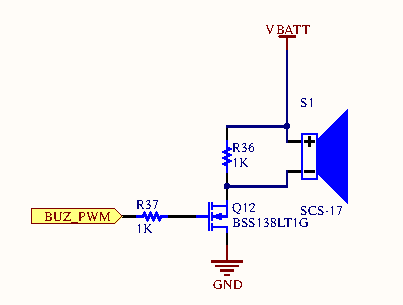
\includegraphics[width=.6\linewidth]{graphics/buzzer_circuit.pdf}
	\caption{Schematic of drive circuit for piezo speaker.}
	\label{fig:buzzer_circuit}
\end{figure}

A MOSFET controlled by a PWM pin is toggling current from VBATT to GND and thereby controlling the sound generated by the piezo.
By changing the dutycycle of the PWM signal the volume produced can be controlled. 
A 50\% dutycycle yields the highest volume. 
A resistor is placed in parallel with the piezo speaker as it is capacitive and needs to discharge when the MOSFET goes off.
The resistor in front of the MOSFET is needed to limit the current from the PWM port. 

In experiments with the circuit and the piezo speaker, the PWM port was connected to a frequency generator set up to do frequency sweeps.
This produced loud and clear clicks.

\subsubsection*{Miniature speaker}
The miniature speaker, as the piezo speaker, needs a drive circuit. 
The circuit from figure \ref{fig:buzzer_circuit} was used again and the same frequency generator was used. 
In this setup the miniature speaker also produces clicks that was audible, but the sounds produces was of significantly lower volume.
Which was also expected.  

\subsubsection*{Conclusion}
It was chosen to use the Piezo speaker with the developed drive circuit as it has the capability of producing a click sound and it produced a significantly greater volume than the miniature speaker in the same setup. 
Besides that it produces no electro magnetic noise as the miniature speaker does. 

\subsection{PWM Generation} % (fold)
\label{sub:pwm_generation}
The Raspberry Pi previously used has support only for one PWM channel.
In order to fully control the robot, four channels are required.
For this reason it was chosen to use an external PWM generator which can be communicated with through I2C.
Moving to an FPGA based platform, this is no longer necessary, as it is possible to add as many PWM channels as required in VHDL\@.
% subsection pwm_generation (end)

\subsection{Motor Driver} % (fold)
\label{sub:motor_driver}
The BD6222HFP was chosen as the motor driver in the previous project.
This is a full-bridge capable of continuously supplying sufficient power to drive the motors on the robot.
While the driver is maintained, a new board will have to be devised to house this driver.
% subsection motor_driver (end)

\subsection{Power and Current limitations} % (fold)
\label{sub:power_and_current_limitations}
It was chosen to use linear regulators to supply the 5 and 3.3V rails.
This project will analyse whether the added cost of using switch-mode converters is worth the additional cost.
A number of fuses were added to limit the current to the motors as well as the current draw from the battery.
The battery however, includes a ``safety board'' which limits the maximum possible current draw, making this fuse irrelevant.
The fuses on the motors can be excluded by instead running a check in software such that when a voltage is applied, the encoder signal must represent movement, or the voltage will be cut.
Allowing overcurrent for a short period will not damage the motors and therefore this approach is acceptable.
% subsection power_and_current_limitations (end)

\subsection{Electronics Board} % (fold)
\label{sub:electronics_board}
In order to accommodate the new electronics a new board will have to be designed.
The board must support a number of components and circuits, listed below.
\begin{itemize}
	\item \textbf{Motor controller:} The BD6222HFP, a full-bridge motor controller, is used to generate the drive signals for the motors.
	\item \textbf{Piezo:} Generating a click is done using a piezo transducer.
	A transducer with an internal drive circuit will be used.
	\item \textbf{5V DC/DC Converter:} The PTH08080W will be used to generate the 5V rail necessary to drive the embedded platform. I provides up to 2.25[A].
	\item \textbf{Connections:} A number of connections has to be present on the board.
	Passthrough for the microphone add-in board.
	Passthrough for the motor encoders.
	Connection for battery.
	\item \textbf{Debug LEDs:} Support for four LEDs for debugging is required.
	The necessary drive circuitry must be added.
	\item \textbf{Microphone board} ....
\end{itemize}

% subsection electronics_board (end)

\subsection{Power Calculations} % (fold)
\label{sub:power_calculations}

\subsubsection{5 [V] rail} % (fold)

% subsection subsection_name (end)
Running at 5[V]:
\begin{itemize}
	\item Microphones including circuitry, $11$[mA]
	\item SBC, $500$[mA]
	\item Two microcontrollers, $5$[mA]
	\item Six LED channels, $120$[mA]
\end{itemize}

Resulting in a total of $636$ [mA] being drawn from the 5[V] rail.

\subsubsection{Battery rail} % (fold)

Only the motor will be running directly off the battery rail.
To measure the current drawn by the motors a small test was conducted.
Three different voltages were applied to the motors by a power supply. 
The results are shown in table \ref{tab:motor_power}.

\begin{table}[]
\centering
\caption{My caption}
\label{tab:motor_power}
\begin{tabular}{|l|l|l|}
\hline
\textbf{Description} & Voltage, [V]   & Current, [mA]      \\ \hline
Barely driving       & 1  & 220  \\ \hline
Medium driving speed & 5  & 305  \\ \hline
Fast driving         & 8  & 350  \\ \hline
\end{tabular}
\end{table}


\subsubsection{Power Dissipation} % (fold)
\label{sec:power_dissipation}
When using a linear voltage regulator the power dissipation is as follows:
$$P_d = (V_{in} - V_{out}) \cdot I_{load}$$
In the average case the battery voltage is thought to be the the nominal voltage, using the found drawn current at 5[V] the power dissipation is found.
$$P_{lr} = (7.4 [V] - 5.0 [V]) \cdot 0.636 [A] = 1.5 [W]$$

If a switching regulator is used the voltage conversion will happen at a significantly higher efficiency.
The pth08080w has a typical efficiency of $93.5\%$ at 5 [V].
The power dissipated in that would be:
$$7.4 [V] \cdot 0.636 [A] \cdot 0.065 = 0.3 [W]$$


The power dissipated at the 5 [V] rail is:
$$P_{5V} = 0.636 [A] \cdot 5 [V] = 3.18 [W]$$

The power dissipated in the motor and motor controller is as in table \ref{tab:power_motor}.

\begin{table}[H]
\centering
\caption{My caption}
\label{tab:power_motor}
\begin{tabular}{|l|l|}
\hline
\textbf{Description} & Power, [W]     \\ \hline
Barely driving       & 0.2 \\ \hline
Medium driving speed & 1.5 \\ \hline
Fast driving         & 2.8 \\ \hline
\end{tabular}
\end{table}

The batteries have a capacity of $2600$ [mAH], giving the following driving times.


\begin{table}[H]
\centering
\caption{My caption}
\label{my-label}
\begin{tabular}{|l|l|p{2cm}|p{2cm}|p{2cm}|p{2cm}|}
\hline
\textbf{Description} & $P_{tot}$ w. LR, {[}W{]} & $P_{tot}$ w. sw, {[}W{]} & Drive time w. LR & Drive time w.  switch& \% more drive time \\ \hline
Barely driving       & 4.9                         & 3.7                               & 3.9              & 5.2                      & 33                 \\ \hline
Medium driving speed & 6.2                         & 5                                 & 3.1              & 3.8                      & 23                 \\ \hline
Fast driving         & 7.5                         & 6.3                               & 2.6              & 3.1                      & 19                 \\ \hline
\end{tabular}
\end{table}

% subsection power_calculations (end)
% section analysis (end)